%%%%%%%%%%%%%%%%%%%%%%%%%%%%%%%%%%%%%%%%%%%%%%%%%%%%%%%%%%%%%%%%%%%%%%%%%%%%%%%%
% setup.tex
% Main tex file for setup and content collocation
% For the use of University of Amsterdam
% Information Systems and Data Science students
% Adapted by Riccardo Fiorista (riccardo.fiorista@proton.me)
%%%%%%%%%%%%%%%%%%%%%%%%%%%%%%%%%%%%%%%%%%%%%%%%%%%%%%%%%%%%%%%%%%%%%%%%%%%%%%%%

% Options:
% Choose one of:
%% `is` - Information Systems
%% `ds` - Data Science 
% Add (separated by `,`):
%% `nolinenumbering` - If you want to remove line numbering on submission
%% `draftmargins` - If you would like to give your reviewer more space for comments
%% `nofrontpicture` - If you do not wish to have a graphic on your front-page
%% `nofirstcompanypicture` - If you do not wish to have a graphic on your front-page
%% `nosecondcompanypicture` - If you do not wish to have a graphic on your front-page
\documentclass[ds,nofirstcompanypicture,nolinenumbering]{mscthesis}

%%%%%%%%%%%%%%%%%%%%%%%%%%%%%%%%%%%%%%%%%%%%%%%%%%%%%%%%%%%%%%%%%%%%%%%%%%%%%%%%
% DOCUMENT METADATA
%%%%%%%%%%%%%%%%%%%%%%%%%%%%%%%%%%%%%%%%%%%%%%%%%%%%%%%%%%%%%%%%%%%%%%%%%%%%%%%%

% Thesis related entries
\title{Simulation-based inference of gravitational waves}
\subtitle{Assessing performance with state-of-the-art deep-learning models}

% Date on which your thesis is submitted
\date{30.06.2024}

% 4-5 keywords should do the trick. They should ideally be phrases of 2-4 words or single words.
\keywords{Simulation-Based Inference, Bayesian Inference, Gravitational Waves, U-Net, Attention U-Net, Vision Transformer, Time Series}

% Author data
\authorname{Nicola Asquith}
\authorid{15058050}
\authoremail{nicola.asquith@student.uva.nl}

% Supervisors
\uvasupervisorname{Associate Professor, Christoph Weniger}
\uvasupervisoraffiliation{GRAPPA Institute for Theoretical Physics}
\uvasupervisoremail{C.Weniger@uva.nl}

% Comment if you do not have an external supervisor
% \externalsupervisorname{External Supervisor} \externalsupervisoraffiliation{External Supervisor}
% \externalsupervisoremail{supervisor@company.nl}

% % Uncomment and fill paths if you want to add custom images
% %% Figure size suggestions (in general it's best to render them from SVGs):
% %% 3000x3000 @ 240dpi for all three
% \titlepicturepath{}
% \firstcompanypicturepath{}
% \secondcompanypicture{path}
\usepackage{csquotes}
\usepackage{placeins}
\usepackage{afterpage}
\usepackage{adjustbox}
%\usepackage[all]{nowidow}
%\widowpenalty10000
%\clubpenalty10000

% Define a new command that uses the length variable
\newcommand{\myvspacecommand}{\vspace{-0.0cm}}

%%%%%%%%%%%%%%%%%%%%%%%%%%%%%%%%%%%%%%%%%%%%%%%%%%%%%%%%%%%%%%%%%%%%%%%%%%%%%%%%
% tikz library
%%%%%%%%%%%%%%%%%%%%%%%%%%%%%%%%%%%%%%%%%%%%%%%%%%%%%%%%%%%%%%%%%%%%%%%%%%%%%%%%
\usepackage{tikz}
\usetikzlibrary{shapes.geometric, arrows}

% Peregrine method

\tikzstyle{sample} = [rectangle, rounded corners, minimum width=1cm, minimum height=1cm, text centered, text width=4cm, draw=black, fill=red!30]
\tikzstyle{simulator} = [rectangle, rounded corners, minimum width=1cm, minimum height=1cm, text centered, text width=4cm, draw=black, fill=blue!30]
\tikzstyle{network} = [rectangle, rounded corners, minimum width=1cm, minimum height=1cm, text centered, text width=5cm, draw=black, fill=green!30]
\tikzstyle{inference} = [rectangle, rounded corners, minimum width=1cm, minimum height=1cm, text centered, text width=2cm, draw=black, fill=yellow!40]
\tikzstyle{pinput} = [rectangle, minimum width=1cm, minimum height=1cm, text centered, draw=black, text width=2cm, fill=pink!30]
\tikzstyle{tinput} = [rectangle, minimum width=1cm, minimum height=1cm, text centered, text width=2cm, draw=black, fill=pink!30]
\tikzstyle{output} = [rectangle, minimum width=1cm, minimum height=1cm, text centered, draw=black, fill=orange!30]

\tikzstyle{arrow} = [thick, ->, >=stealth]

% UNet architecture

\tikzstyle{input} = [rectangle, minimum width=1cm, minimum height=0.1cm, text centered, draw=white, fill=white!30]
\tikzstyle{conv} = [rectangle, minimum width=1cm, minimum height=0.1cm, text centered, draw=black, fill=orange!30]
\tikzstyle{convx2} = [rectangle, minimum width=1cm, minimum height=0.1cm, text centered, draw=black, fill=orange!30]
\tikzstyle{pool} = [rectangle, minimum width=1cm, minimum height=0.1cm, text centered, draw=black, fill=blue!30]
\tikzstyle{upconv} = [rectangle, minimum width=1cm, minimum height=0.1cm, text centered, draw=black, fill=green!30]
\tikzstyle{concat} = [rectangle, dotted, minimum width=1cm, minimum height=0.1cm, text centered, draw=black, fill=white!30]
\tikzstyle{outconv} = [rectangle, minimum width=1cm, minimum height=0.1cm, text centered, draw=black, fill=orange!30]
\tikzstyle{flatten} = [rectangle, minimum width=1cm, minimum height=0.1cm, text centered, draw=black, fill=lime!30]
\tikzstyle{fc} = [rectangle, minimum width=1cm, minimum height=0.1cm, text centered, draw=black, fill=red!30]
\tikzstyle{summary} = [ellipse, minimum width=1cm, minimum height=0.1cm, text centered, text width=1.5cm, draw=black, fill=teal!30]
\tikzstyle{AG} = [circle, dashed, minimum width=0.1cm, minimum height=0.1cm, text centered, draw=black, fill=violet!30]

\tikzstyle{arrow_unet} = [thin, ->, >=stealth]
\tikzstyle{arrow_unet_dotted} = [dashed, thin, ->, >=stealth]

% Peregrine architecture

\tikzstyle{per_input} = [rectangle, minimum width=1cm, minimum height=0.1cm, text centered, draw=black, fill=blue!30]
\tikzstyle{per_unet} = [rectangle, minimum width=1cm, minimum height=0.1cm, text centered, draw=black, fill=red!30]
\tikzstyle{per_features} = [rectangle, minimum width=1cm, minimum height=0.1cm, text centered, draw=black, fill=green!30]
\tikzstyle{per_concat} = [rectangle, dotted, minimum width=1cm, minimum height=0.1cm, text centered, draw=black, fill=white!30]
\tikzstyle{per_MLP} = [rectangle, minimum width=1cm, minimum height=0.1cm, text centered, draw=black, fill=orange!30]
\tikzstyle{per_labels} = [rectangle, minimum width=1cm, minimum height=0.1cm, text centered, draw=black, fill=cyan!30]
\tikzstyle{per_logratios} = [rectangle, minimum width=1cm, minimum height=0.1cm, text centered, draw=black, fill=magenta!30]

% Attention gate

\tikzstyle{wg} = [rectangle, text centered, draw=black, fill=blue!30]
\tikzstyle{wx} = [rectangle, text centered, draw=black, fill=blue!30]
\tikzstyle{plus} = [circle, text centered,  text width=0.2cm, draw=black, fill=white!30]
\tikzstyle{relu} = [rectangle, text centered, draw=black, fill=white!30]
\tikzstyle{psi} = [rectangle, text centered, draw=black, fill=blue!30]
\tikzstyle{sigmoid} = [rectangle, text centered, draw=black, fill=white!30]
\tikzstyle{times} = [circle, text centered, text width=0.2cm, draw=black, fill=white!30]

%%%%%%%%%%%%%%%%%%%%%%%%%%%%%%%%%%%%%%%%%%%%%%%%%%%%%%%%%%%%%%%%%%%%%%%%%%%%%%%%
% CONTENT
%%%%%%%%%%%%%%%%%%%%%%%%%%%%%%%%%%%%%%%%%%%%%%%%%%%%%%%%%%%%%%%%%%%%%%%%%%%%%%%%

\begin{document}
\pagestyle{plain}

\maketitlepage
\fixemptypage
\setcounter{page}{1}

\begin{abstract}
% A summary of results should be included. Avoid citations. Maximum length is 200 words.

The detection and analysis of gravitational waves (GW) allows scientists to study the universe from a new perspective. Current techniques for parameter inference of GW are computationally expensive, and the substantial increase in detected events expected in the future is introducing significant data analytics challenges for the GW community. The \texttt{peregrine} analysis pipeline implements multiple sequential rounds of simulation-based inference with the U-Net CNN architecture. While this pipeline successfully performs high precision GW parameter inference, the network training time is a significant bottleneck.
In this work, we assessed several modifications of the \texttt{peregrine} pipeline, with the aim to improve the overall performance. Attention mechanisms, particularly as applied in transformer models have become very popular in recent years due to their reported high performance. We compare the performance of \texttt{peregrine} with the baseline U-Net model with several variations, including Attention U-Net, pre-trained vision transformer, pre-trained multi-variate time series transformer, and finally, structured network pruning of the original U-Net. After a thorough investigation of the most promising state-of-the-art techniques, we concluded that the original U-Net in \texttt{peregrine} is already close to optimal.

%we found no convincing evidence that these modifications improve the performance of .

%that the best performing model was the original U-Net, and that the use of larger transformer models did not provide any performance improvement. This was predominantly due to longer training times required. The pruned networks could be trained faster but suffered from poorer accuracy in later inference rounds.

\end{abstract}

\maketitle

%\stepcounter{footnote}
%\footnotetext{Github Repository: \url{}

\section*{Github Repository}
\url{https://github.com/Nic0laA/master-thesis}

% Sections; Try to stick to this setup but you can comment each section
\section{Introduction}
\label{sec:introduction}
% Mention scientific context/field, problem statement, research gap and candidate (sub) research question(s). 

Gravitational Waves (GW) are ripples in the fabric of space-time originating from the acceleration of massive astronomical objects e.g. the merger of black holes or neutron stars. 
Analysis of gravitational waves can be used to infer physical information regarding their source of origin, as well as provide the opportunity to observe the universe in an entirely new way.

Since the first direct detection of gravitational waves in 2015 \cite{LIGO_2016}, the detector sensitivities and survey volumes are ever-increasing. The substantial rise in detection rate of events over time is introducing significant data analysis challenges for the gravitational wave community \cite{bhardwaj2023peregrine}.
For instance, current data analysis pipelines are not equipped to deal with independent signals arriving coincidentally in detectors, and scale poorly as the dimensionality of the problem increases \cite{alvey2023things}. This makes the analysis of large number of overlapping signals, or those containing non-stationary noise increasingly complicated and computationally expensive \cite{bhardwaj2023peregrine}.

The \texttt{peregrine} inference pipeline has been developed at the UvA GRAPPA institute to help address some of these challenges \cite{bhardwaj2023peregrine}. It utilises the Simulation-based inference (SBI) method based on the TMNRE (Truncated Marginal Neural Ratio Estimation) algorithm with the U-Net Convolutional Neural Network (CNN) architecture. The \texttt{peregrine} pipeline consists of multiple rounds of network training and inference, which comes with a high simulation cost. It is therefore highly beneficial for the network to be as fast and as accurate as possible. This thesis explores the possibilities to optimise the network architecture underlying the \texttt{peregrine} code. The main research question will be: 

\noindent \textit{RQ: To what extent can the optimisation of the \texttt{peregrine} network architecture reduce the simulation budget, while still producing the same results as the original \texttt{peregrine}?}

Smaller sub-questions to be addressed include:

\noindent SRQ1: How can we quantify the efficiency of the underlying neural network?

\noindent SRQ2: How can more efficient sampling methods be used to further improve the computational efficiency of \texttt{peregrine}?

To explore the possibilities of improving the performance of the U-Net CNN within \texttt{peregrine}, we will consider two competing approaches - expansion and reduction. For the expansion part, we will look at two pretrained vision transformer models \cite{Dosovitskiy_2021_ViT,Zerveas_2020_mvts}, and attention u-net \cite{Oktay_2018_AUNet}. For the reduction approach, we will look at pruning methods \cite{Fang_Ma_Song_Mi_Wang_2023}.

The structure of this report is as follows. Related work in section bla, background theory in section bla.
\section{Related Work}
\label{sec:related_work}
% Your work needs to be grounded and compared to earlier work and the state-of-the-art. Start the section with announcing the research gap and also end with the research gap. Consider using hypotheses. 

\subsection{Gravitational Wave analysis}

The first direct detection of gravitational waves occurred in 2015 after the merger of two black holes about 1.3 billion light years away~\cite{LIGO_2016}. Since then, there have been three observing runs by the LIGO-Virgo collaboration which have yielded 90 confirmed gravitational wave detections . Of these 90 detections, 83 were binary black hole mergers, 2 were binary neutron star mergers, 3 were neutron star-black hole mergers and 2 involved the merger between a black hole and a `mystery' object that had a mass in between that of a neutron star and black hole~\cite{LIGO_FAQ_Website}. The next observing runs, O4 (started May 2023) and O5 (planned for 2027 and beyond) are predicted to detect a significant increase in events (${\sim}5\times$ more events each corresponding observing run~\cite{Petrov_2022}).

Analysis of gravitational waves is divided into two parts -- detection using highly sensitive laser interferometers, and parameter inference~\cite{bhardwaj2023peregrine}. In this work, we consider only the inference part. That is, given an observed GW waveform, how can we infer the physical properties of the source, as well as the distance, position and orientation of the source in the sky relative to the observation etc.

Given well-established methods, it is currently straight-forward to (forward) simulate a gravitational wave signal. The theory of how sources emit gravitational waves is well known, and the entire gravitational waveform may be expressed by $\sim$15 parameters~\cite{Thrane_Talbot_2019}. In addition, we can accurately model detector responses and instrument noise~\cite{alvey2023things} using e.g.~the open-source Bilby code~\cite{Ashton_Bilby_2019,Romero_Bilby_2020,Ashton_Talbot_Bilby_2021}. However, despite having access to high-fidelity simulators, these simulators alone are poorly suited to statistical inference and lead to challenging inverse problems, since the likelihoods for a given observation is intractable~\cite{Cranmer_SBI_2020}. In other words, backing out the 15 input parameters from a given GW waveform is significantly more challenging than forward simulating the generation of that same waveform.

Due to the high dimensionality, brute-force techniques for GW parameter inference are computationally infeasible. The traditional approach involves using stochastic sampling methods~\cite{Thrane_Talbot_2019}, such as Markov chain Monte Carlo (MCMC)~\cite{Metropolis_1953,Hastings_1970} or nested sampling~\cite{Skilling_2004}. However, these techniques increasingly struggle with higher dimensional data and are not feasible options in the case of overlapping signals, where one needs to now infer 30 model parameters from the data~\cite{alvey2023things}.

Simulation-based inference (SBI), or likelihood-free inference, has proven to be an effective technique for performing statistical inference in situations where the likelihood is intractable. SBI is a machine-learning method that combines a forward simulator, a statistical surrogate model and set of prior beliefs. It outputs approximate posterior distributions of parameters given some observed data~\cite{Miller2022}. The likelihoods can be sampled implicitly from data generated using a high-fidelity forward simulator. SBI has undergone rapid expansion in recent years, thanks to the enormous rise in machine learning capabilities~\cite{Cranmer_SBI_2020}. It is considered to be a highly simulation efficient technique and finds applications in many scientific domains including particle physics, neuroscience, epidemiology, economics, climate science and astrophysics~\cite{Cranmer_SBI_2020}.

\subsection{Swyft and Peregrine}

\texttt{swyft} is a python package that implements a simulation-efficient SBI algorithm known as Truncated Marginal Neural Ratio Estimation (TMNRE) (described in section~\ref{sec:tmnre}). It calculates likelihood-to-evidence ratios to approximate marginal posteriors for parameters of interest. A collection of tools to efficiently simulate and store data (using zarr storage~\cite{Miles_zarr_2021}), as well as the framework to integrate PyTorch models~\cite{paszke2019pytorch} are incorporated into the \texttt{swyft} library~\cite{Miller2022}.

The \texttt{Peregrine} code has been built on-top of the \texttt{swyft} library. It was developed to study broad classes of gravitational wave signals. The papers describing the development of the code~\cite{bhardwaj2023peregrine,alvey2023things} form the starting point of this thesis, and also serve as the baseline for this work to be benchmarked against. Details of \texttt{Peregrine} are given in section~\ref{sec:methodology_peregrine}.

\subsection{U-Net}

\subsubsection{Original U-Net}

U-Net is a fully convolutional neural network that was originally developed in 2015 for biomedical image segmentation~\cite{Ronneberger_Fischer_Brox_2015}. U-Net is efficient and fast to train, leading it to become highly popular and it may even be considered the \enquote{gold standard} for 2D medical image segmentation~\cite{Sengara_2022}. The defining feature of U-Net is its symmetrical U-shaped architecture consisting of a contracting path (encoder) followed by an expansive path (decoder). The encoding path captures the context and features in the image, while the decoding path reconstructs the image back to its original resolution from the extracted features to segment the image into different classes. Linking the encoding and decoding paths is the bottleneck, which is the deepest part of the network containing the highest number of feature channels and lowest spatial resolution.

In the original U-Net~\cite{Ronneberger_Fischer_Brox_2015}, each step in the encoding path consists of two 3$\times$3 convolutions (unpadded in the original) with a ReLU activation function, doubling the number of feature channels, and 2$\times$2 max pooling with stride 2 for downsampling the spatial dimensions. The decoding path then follows with a 2$\times$2 \enquote{up-convolution} halving the number of feature channels, concatenation with the matching feature map from the encoder path (skip connection), followed by two 3$\times$3 convolutions and ReLU operations. The architecture of U-Net, reproduced from~\cite{Ronneberger_Fischer_Brox_2015}, is shown in Figure~\ref{fig:unet_arch}.

\begin{figure}[tb]
    \centering
    \includegraphics[width=1\linewidth]{media/images/UNet_arch.png}
    \caption{The U-Net architecture with a 2D image of resolution 572$\times$572 as example input. Image reproduced from~\cite{Ronneberger_Fischer_Brox_2015}.}
    \Description[<short description>]{<long description>}
    \label{fig:unet_arch}
    \myvspacecommand
\end{figure}

\subsubsection{Attention U-Net}

Attention U-Net extends the original U-Net architecture with the addition of an attention mechanism. This is claimed to improve the sensitivity and prediction accuracy of the network, with minimal impact to the computational cost~\cite{Oktay_2018_AUNet}. The attention mechanism consists of attention gates that filter the features transmitted through the skip connections. This applies additive soft attention to help the network learn to suppress irrelevant features and focus only on the most important features in the image.

In addition to Attention U-Net, several other variants of U-Net have also been proposed in the literature. This includes Residual U-Net~\cite{Zhang_resunet_2018}, Dense U-Net~\cite{Wang_dense_unet_2019}, R2U-Net~\cite{Alom_r2unet_2018}, U-Net++~\cite{Zhou_2018_unet++} and TransUNet~\cite{Chen_transunet_2021}. We chose to test the Attention U-Net with \texttt{peregrine} since it is the most popular variant (based on the number of article citations at present time), and due to the authors claim that the performance is enhanced without adding additional computational burden.

% U-Net++ replaces the plane skip connections in vanilla U-Net with nested dense skip connections. This is to reduce the semantic gap between the encoder and decoder, which they claim yields significant performance gains.

\subsection{Transformer models}

\subsubsection{Vision Transformer}

Transformer models have revolutionized the field of NLP (Natural Language Processing) with their self-attention mechanisms that do not rely on recurrence or convolutions~\cite{Vaswani_2017_transformer}. Transformer models can also be applied to image recognition tasks, where the image is divided into a sequence of patches. Positional embeddings are combined with the patch embeddings to store the positional information. It has been demonstrated that Vision Transformer models can match, and even outperform state-of-the-art CNN for image classification tasks~\cite{Dosovitskiy_2021_ViT}. The self-attention mechanism of the transformer allows the model to focus on the most relevant parts of the image, which capture the longer-range dependencies more effectively than RNNs or CNNs. Due to the reported high performance of the Vision Transformer over conventional CNN, we would like to test the performance of a Vision Transformer model compared to the U-Net CNN within \texttt{Peregrine}.

The main drawback with transformers in general, is their higher complexity compared to CNNs. This means they require more computational resources (e.g. more RAM, GPUs/TPUs), longer training times and more training data. Pretraining transformers on large amounts of training data to learn general representations, and then fine-tuning them with a smaller amount of task-specific data can be a way to achieve high performance using less computational resources~\cite{Tay_Dehghani_Rao_Fedus_Abnar_Chung_Narang_Yogatama_Vaswani_Metzler_2022}.

\subsubsection{Multi-variate Time Series Transformer}

The success of the transformer models in the NLP and computer vision fields, has attracted great interest in the time-series community~\cite{Wen_Zhou_Zhang_Chen_Ma_Yan_Sun_2023}. Transformers are particularly suited to time series data due to their ability to capture longer-range dependencies. They have been shown to be effective feature extractors in 1D signals~\cite{Nguyen_Miah_Bilodeau_Bouachir_2022}. In ~\cite{Nguyen_Miah_Bilodeau_Bouachir_2022}, the time signal was divided into segments and the encoder part of the traditional transformer used in NLP was used to extract relevant features. The resulting model outperformed state-of-the-art algorithms (in 2022) for detection of Parkinson's disease from signals of a patients gait. 

We have chosen to utilise the multivariate time series (MTS) transformer-based framework proposed for unsupervised representation learning~\cite{Zerveas_2020_mvts}. The authors claim that their approach outperforms all state-of-the-art (as of 2020) supervised methods, by a significant margin, even with limited training data. After pretraining the transformer to extract dense vector representations of the time series through an autoregressive objective, the model can then be applied to downstream tasks such as regression, classification, imputation and forecasting. Due to the claimed performance of this model, we think it is a potential alternative to U-Net. The main difference between the MTS model and the ViT model, is that the MTS has been specifically tailored to focus on sequential patterns, while the ViT focuses on visual features within images.

\subsection{Network pruning}

The Attention U-Net and transformers models will increase the complexity compared to the original U-Net that is currently in \texttt{Peregrine}. Even with the potential accuracy increase, the larger networks will place a heavier burden on computational resources and/or require more training data. In order to reduce the number of trainable parameters in the current U-Net, with the intent to decrease the training time, we will investigate whether structural network pruning techniques yield any benefit. Pruning networks has proven itself to be a practical and effective way of compressing networks, as it can help to accelerate inference by removing redundant parameters. Specifically, DepGraph (Dependency Graph), is an automatic method to model residual connections and dependencies between paired layers so groups of parameters can be pruned in a structured way~\cite{Fang_Ma_Song_Mi_Wang_2023}.

%\section{Background Theory}
\label{sec:background_theory}

\subsection{Simulation-based inference}
\label{sec:background_theory_sbi}





\section{Methodology}
\label{sec:methodology}
% Focus on what you add to the existing method. Explain what you will do and why (and how). Do not forget to characterize your research design. There should be an evaluation plan in this section. (For DS students, this normally means using manually labelled or ground truth data.)

\todo[inline]{Very much still a work in progress}

% ============================================================================ %
% Description of the data
% ============================================================================ %
\subsection{Description of the data}

The data used in this study was simulated using the open-source Bilby code~\cite{Ashton_Bilby_2019}. The gravitational waveforms of three LIGO detectors (Hanford, Washington and Livingston) were generated as a function of 15 independent parameters. Ten of these parameters represented intrinsic properties of the source e.g. the masses and spins of the two black holes, while five of these are extrinsic parameters e.g. the distance from the source and orientation in the sky with respect to the observations. Further details of the parameters are listed in Table~\ref{tab:gw_parameters}. Simulating the waveforms for training the neural network is necessary since we need $\sim$100000 waveforms for training and experimentally measured signals are rare (only 90 detections so far).

Only low SNR case considered because high SNR is unrealistic and it is important for the network to determine signal from noise.

\todo[inline]{Complete table}

\begin{table}[htb]
\centering
\begin{tabular}{|l|l|l|l|}
\hline
\textbf{Parameter} & \textbf{Type} & \textbf{Prior} & \textbf{Test Value} \\
\hline
Mass ratio, \( q \) & I & \( U(0.125, 1) \) & 0.8858 \\
Chirp mass \( M \) [\( M_{\odot} \)] & I & \( U(25, 100) \) & 32.14 \\
Inclination angle \( \theta_{jn} \) [rad] & I & sine(0, \( \pi \)) & 0.4432 \\
Phase \( \phi_c \) [rad] & I & \( U(0, 2\pi) \) & 5.089 \\
Tilt angle \( \theta_1 \) [rad] & I & sine(0, \( \pi \)) & 1.497 \\
Tilt angle \( \theta_2 \) [rad] & I & sine(0, \( \pi \)) & 1.102 \\
Spin \( a_1 \) & I & \( U(0.05, 1) \) & 0.9702 \\
Spin \( a_2 \) & I & \( U(0.05, 1) \) & 0.8118 \\
Spin angle \( \phi_{12} \) [rad] & I & \( U(0, 2\pi) \) & 6.220 \\
Spin angle \( \phi_{jl} \) [rad] & I & \( U(0, 2\pi) \) & 1.885 \\
Luminosity Distance \( d_L \) [Mpc] & E & \( U_{\text{vol}}(100, 2000) \) & 900 \\
Right ascension \( \alpha \) [rad] & E & \( U(0, 2\pi) \) & 5.556 \\
Declination \( \delta \) [rad] & E & cosine(-\( \pi/2 \), \( \pi/2 \)) & 0.071 \\
Polarisation angle \( \psi \) [rad] & E & \( U(0, \pi) \) & 1.100 \\
Merger time \( t_c \) [GPS s] & E & \( U(-0.1, 0.1) \) & 0.000 \\
\hline
\end{tabular}
\caption{Description and type of the parameters that fully describe the detected gravitational waves.}
\label{tab:gw_parameters}
\end{table}

The waveform data consists of 1D signals in both time and frequency domains, collected from the three separate detectors that have captured the event simultaneously. An example of the signal in the time domain is shown in Figure~\ref{fig:obs_time_domain}. In total, there are 8192 channels corresponding to 4\,s of collection time at a sampling frequency of 2048\,Hz. With the Fourier transform, the time signal is decomposed into its constituent frequency components. Both the time and frequency domains are fed into the neural network, since they have different information about the parameters encoded. An example of the signal in the frequency domain is shown in Figure~\ref{fig:obs_freq_domain}.

\begin{figure}
  \centering
  \includegraphics[width=1\linewidth]{media/images/obs_time_domain_lowSNR.png}
  \caption{Example of generated gravitational wave signal in the time domain. Signals from three detectors are shown. For clarity, the noise and signal are shown separately in the figure, but are added together when training the network. The two black holes merge at the moment t=0s. }
  \label{fig:obs_time_domain}
\end{figure}

\begin{figure}
  \centering
  \includegraphics[width=1\linewidth]{media/images/obs_freq_domain_lowSNR.png}
  \caption{Example of generated gravitational wave signal in the frequency domain. Signals from three detectors are shown. For clarity, the noise and signal are shown separately in the figure, but are added together when training the network.}
  \label{fig:obs_freq_domain}
\end{figure}

Only low signal to noise signal will be considered here since the high SNR is unphysical and the low SNR is more challenging. Many moving parts to problem - number of truncation rounds, the number of simulations per round, network architecture, the truncation, the sampling strategy of the priors.

% ============================================================================ %
% Peregrine
% ============================================================================ %
\subsection{Peregrine inference pipeline}

The overall objective of this work is to increase the efficiency of the \texttt{Peregrine} data analysis pipeline. The work will begin with reproducing the results from papers~\cite{bhardwaj2023peregrine} and~\cite{alvey2023things}, as this will form the benchmark to which the eventual results will be compared to.

The workflow for the simulation-based inference technique for the analysis of the gravitational wave signals as implemented in \texttt{peregrine}~\cite{bhardwaj2023peregrine} is shown in Figure~\ref{fig:peregrine_pipeline}. The process starts by setting the 15 parameters of the `target observation' and then generating the example waveform to be analysed. This is done so there are `ground-truth' parameter values that you can compare your final posterior probability density distributions with and validate the overall method. If we use a true experimentally measured signal, then we can never know for certain what the `ground-truth' values of the parameters are. Given the accuracy that we can forward model the GW signals with, once the method is validated with the simulated waveforms, it is expected to work equally well with true experimental measurements.

\begin{figure}[htb]
    \centering
    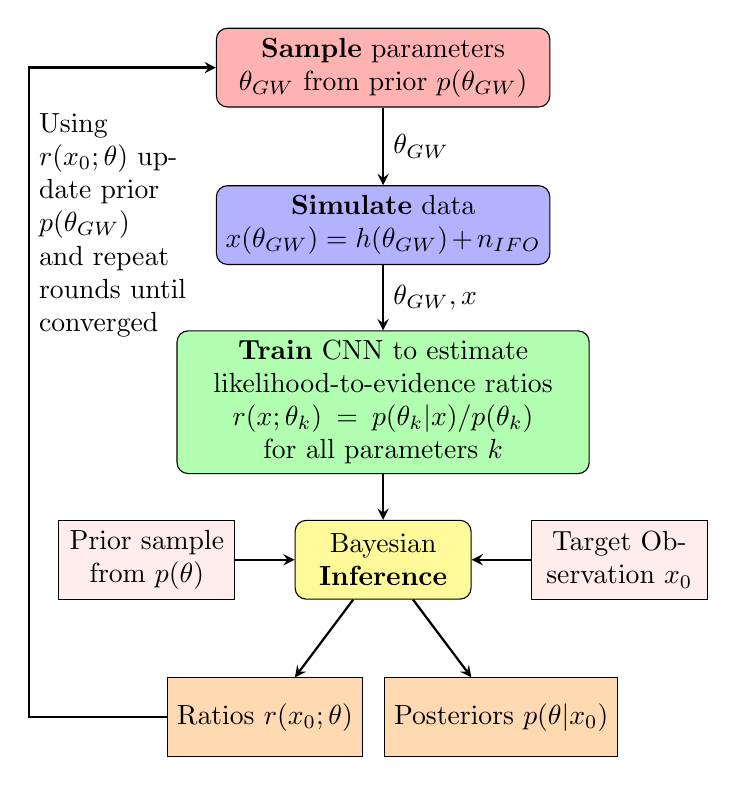
\begin{tikzpicture}[node distance=2cm]
        \node (sampling) [sample] {\textbf{Sample} parameters $\boldsymbol{\theta}_{GW}$ from prior $p(\boldsymbol{\theta}_{GW})$};
        \node (fsimulator) [simulator, below of=sampling] {\textbf{Simulate} data $\boldsymbol{x}(\theta_{GW}) = h(\theta_{GW}) + n_{IFO}$};
        \node (network) [network, below of=fsimulator, yshift=-0.25cm] {\textbf{Train} CNN to estimate likelihood-to-evidence ratios $r(\boldsymbol{x};\theta_k) = p(\theta_k|\boldsymbol{x})/p(\theta_k)$ for all parameters $k$};
        \node (inference) [inference, below of=network] {Bayesian \textbf{Inference}};
        \node (prior) [pinput, left of=inference, xshift=-1cm] {Prior sample from $p(\theta)$};
        \node (target) [tinput, right of=inference, xshift=1cm] {Target Observation $\boldsymbol{x}_0$};
        \node (ratios) [output, below of=inference, xshift=-1.5cm] {Ratios $r(\boldsymbol{x}_0;\theta)$};
        \node (posterior) [output, below of=inference, xshift=1.5cm] {Posteriors $p(\theta|\boldsymbol{x}_0)$};
        \draw [arrow] (sampling) -- node[anchor=west] {$\boldsymbol{\theta}_{GW}$} (fsimulator);
        \draw [arrow] (fsimulator) -- node[anchor=west] {$\boldsymbol{\theta}_{GW},\boldsymbol{x}$} (network);
        \draw [arrow] (network) -- (inference);
        \draw [arrow] (prior) -- (inference);
        \draw [arrow] (target) -- (inference);
        \draw [arrow] (inference) -- (posterior);
        \draw [arrow] (inference) -- (ratios);
        \draw [arrow] (ratios) -- +(-3,0) |- node[anchor=west, yshift=-2cm, text width=2cm]{Using $r(\boldsymbol{x}_0;\theta)$ update prior $p(\boldsymbol{\theta}_{GW})$ and repeat rounds until converged} (sampling);
    \end{tikzpicture}
    \caption{High-level overview of the simulation-based inference method used for this work.}
    \label{fig:peregrine_pipeline}
\end{figure}


Fifteen individual binary classifiers. Minimise binary cross-entropy loss.

Noise shuffling.

% \subsection{Optimising of sampling efficiency}

% We will investigate whether some more active learning can be introduced to increase the efficiency of the sampling process. For instance, some parameters such as the chirp mass\footnote{The chirp mass is a combination of the two object masses in the binary system, and is a key factor in the gravitational wave frequency as the two objects spiral inwards toward each other.\\$\mathcal{M} = \frac{(m_1 \cdot m_2)^{3/5}}{(m_1 + m_2)^{1/5}}$} may be inferred early on with relatively high confidence, but currently in successive simulation rounds continues to be sampled from a uniform distribution within $\pm5\sigma$~\cite{Miller_TMNRE_2021}. We will investigate whether it's possible to be more selective in the sampling of parameters that are known with relatively high confidence in an un-biased way. Therefore, we can focus the simulation budget more on the parameters we know with less confidence. To do this in a systematic way, a complete survey of how influential each parameter is on the different segments of the GW signal will be carried-out first.

The current rendition of the Peregrine pipeline requires 8 rounds of sequential TMNRE, 720000 simulated waveforms and around 12.5 hours (on a single A100 gpu with 18 cpu cores) to completely reconstruct the posteriors of the fifteen parameters. Of these 12.5 hours, around 10 is for training the network and 2.3 is for generating the waveforms used for training the network. Our primary focus is therefore the optimisation of the pipeline on the network itself, and as a secondary the number of simulated waveforms.

Trainer settings.

% ============================================================================ %
% Overview
% ============================================================================ %
\subsection{Overview of approach}

Focus on the loss 

% ============================================================================ %
% Transformer models
% ============================================================================ %
\subsection{Transformer models}



\subsubsection{Hyperparameter tuning}

RayTune was used to tune hyperparameters. 

\subsubsection{Pretraining}

Transformers were pretrained for 24 hours with single A100 gpu on 2 million waveforms.


% ============================================================================ %
% Attention U-Net
% ============================================================================ %
\subsection{Attention U-Net}



% ============================================================================ %
% Pruning
% ============================================================================ %
\subsection{Pruning}


%The architecture of the network currently implemented in \texttt{peregrine} is the U-Net architecture~\cite{Ronneberger_UNet_2015}. Given the advances in machine learning and CNN architectures since 2015, it is believed that this network can be improved upon. The optimisation of this network architecture will be the main focus of this thesis. 

%Investigative studies will be performed to find the best network architectures most suitable for the data format. We will first try with LSTM's since they are known to work well with noisy time-series data. The chosen network architecture also needs to be capable of segmenting the signal into three components, representing the different stages of the merger event -- inspiral, merger and ringdown~\cite{Pan_GW_2014}. Each of the parameters in $\boldsymbol{\theta}_{GW}$ are impacted differently in the different phases~\cite{bhardwaj2023peregrine}. Given the network is a binary classifier that classifies between joint and marginally drawn sample pairs, we will assess the performance of the network with the ROC curve.


% ============================================================================ %
% Evaluation
% ============================================================================ %
\subsection{Evaluation}

%The changes to the \texttt{peregrine} analysis pipeline will be fully benchmarked against the original \texttt{peregrine}, both in terms of accuracy of final result and required runtime. The results of the original \texttt{peregrine} have themselves been benchmarked against established likelihood-based methods~\cite{Speagle_2020}, and found to be in good agreement. Therefore, in this work we think it is sufficient to compare only with the original \texttt{peregrine}. To demonstrate the applicability of the method to real gravitational wave measurements, if time permits, we will also test the approach using real experimental data.


\section{Results}
\label{sec:results}
% Give the outcomes for each research question in the form of a table or graphic (with caption).
% Write about your results here. Good captions to tables and/or figures are key.

\subsection{Transformer models}

% Show loss curve of UNet, ViT and MVTS transformer. 
In this section, we show the results during the pretraining of the transformer models

We can conclude that the ViT does not extract any additional features from the data, since the loss plateus to the same value. However, due to extra features the ViT is much slower. The mvts model is not a good model.

The pretrained ViT model was used for the evaluation of Peregrine. Round 2 training of ViT took 11 hours, so was terminated not to waste computing budget.

AUROC for 15 features after 24 hours of training.

\begin{table}
    \caption{Loss values for each of the features}
    \begin{tabular}{lrrr}
    \toprule
    feature & mvts & vit & unet \\
    \midrule
    mass ratio & -0.231 & -0.295 & -0.300 \\
    chirp mass & -0.542 & -0.676 & -0.701 \\
    theta jn & -0.327 & -0.463 & -0.426 \\
    phase & 0.000 & 0.000 & 0.000 \\
    tilt1 & -0.107 & -0.167 & -0.174 \\
    tilt2 & -0.018 & -0.036 & -0.036 \\
    a1 & -0.078 & -0.104 & -0.132 \\
    a2 & -0.005 & -0.008 & -0.007 \\
    phi12 & 0.000 & 0.000 & 0.000 \\
    phijl & -0.199 & -0.291 & -0.287 \\
    luminosity distance & -0.196 & -0.294 & -0.291 \\
    dec & -0.830 & -0.923 & -0.899 \\
    ra & -1.020 & -1.085 & -1.066 \\
    psi & -0.063 & -0.117 & -0.090 \\
    geocent time & -0.965 & -1.104 & -1.105 \\
    \bottomrule
    \end{tabular}
\end{table}

\begin{figure}
  \centering
  \includegraphics[width=1\linewidth]{media/images/Pretraining_loss_curve.png}
  \caption{Bla}
  \label{fig:pretain_loss_curve}
\end{figure}

\subsection{Peregrine Network}

Runtime for the rounds.

\begin{table}
\caption{Network performance of different network architectures for Peregrine}
\begin{tabular}{lrrrrrrr}
\toprule
\multicolumn{1}{p{0.5cm}}{\raggedright Network}  & 
\multicolumn{1}{p{0.5cm}}{\raggedleft Round}  &
\multicolumn{1}{p{1cm}}{\raggedleft Num \\ Epochs} &
\multicolumn{1}{p{1cm}}{\raggedleft Num \\ Steps} &
\multicolumn{1}{p{1cm}}{\raggedleft Sampling \\ Fraction} &
\multicolumn{1}{p{0.75cm}}{\raggedleft Train \\ Loss} &
\multicolumn{1}{p{0.75cm}}{\raggedleft Test \\ Loss} &
\multicolumn{1}{p{1cm}}{\raggedleft Avg \\ AUROC} \\
\midrule
UNet & 1 & 104 & 10504 & 4.98e-03 & -4.71 & -4.22 & 0.706 \\
UNet & 2 & 79 & 16432 & 2.66e-05 & -4.78 & -4.65 & 0.738 \\
UNet & 3 & 77 & 23793 & 2.38e-06 & -4.71 & -4.47 & 0.741 \\
UNet & 4 & 74 & 30858 & 1.61e-06 & -4.14 & -4.43 & 0.741 \\
UNet & 5 & 90 & 37530 & 8.15e-07 & -4.43 & -4.39 & 0.742 \\
UNet & 6 & 60 & 31440 & 6.03e-07 & -4.19 & -4.25 & 0.736 \\
\midrule
Att UNet & 1 & 74 & 7474 & 1.04e-02 & -4.48 & -4.16 & 0.710 \\
Att UNet & 2 & 78 & 16224 & 2.21e-05 & -4.83 & -4.65 & 0.731 \\
Att UNet & 3 & 58 & 17922 & 5.59e-06 & -4.35 & -4.35 & 0.735 \\
Att UNet & 4 & 54 & 22518 & 2.76e-06 & -4.32 & -4.27 & 0.736 \\
Att UNet & 5 & 87 & 36279 & 2.51e-06 & -4.38 & -4.16 & 0.735 \\
Att UNet & 6 & 83 & 43492 & 1.74e-06 & -4.09 & -4.19 & 0.734 \\
\midrule
UNet 5\% & 1 & 68 & 6868 & 4.21e-03 & -5.03 & -4.43 & 0.716 \\
UNet 5\% & 2 & 65 & 13520 & 5.40e-05 & -4.85 & -4.49 & 0.731 \\
UNet 5\% & 3 & 75 & 23175 & 7.71e-06 & -4.05 & -4.33 & 0.736 \\
UNet 5\% & 4 & 48 & 20016 & 4.67e-06 & -4.09 & -4.41 & 0.743 \\
UNet 5\% & 5 & 60 & 25020 & 3.91e-06 & -4.27 & -4.46 & 0.743 \\
UNet 5\% & 6 & 30 & 15720 & 3.52e-06 & -4.74 & -4.38 & 0.741 \\
\midrule
UNet 10\% & 1 & 39 & 3939 & 4.31e-02 & -3.98 & -3.89 & 0.689 \\
UNet 10\% & 2 & 35 & 7280 & 3.72e-03 & -3.67 & -3.76 & 0.706 \\
UNet 10\% & 3 & 58 & 17922 & 4.33e-05 & -4.42 & -4.62 & 0.732 \\
UNet 10\% & 4 & 57 & 23769 & 1.14e-05 & -4.54 & -4.27 & 0.735 \\
UNet 10\% & 5 & 30 & 12510 & 8.17e-06 & -3.90 & -3.96 & 0.725 \\
UNet 10\% & 6 & 56 & 29344 & 4.87e-06 & -4.08 & -4.31 & 0.738 \\
\midrule
ViT & 1 & 30 & 12540 & 4.37e-05 & -6.15 & -5.58 & 0.753 \\
ViT & 2 & 60 & 50460 & 2.03e-06 & -5.82 & -5.28 & 0.757 \\
\bottomrule
\end{tabular}
\end{table}


Look at different parameters for round 6.
Compare the four different UNet models.

\begin{table}
\caption{Round 6 AUC and loss values}
\hspace*{-2cm}
\begin{tabular}{lrrrrrrrr}
\toprule
Param & 
\multicolumn{1}{p{0.3cm}}{\raggedright UNet}  & 
\multicolumn{1}{p{0.3cm}}{\raggedleft Att UNet}  &
\multicolumn{1}{p{0.3cm}}{\raggedleft UNet 10\%}  &
\multicolumn{1}{p{0.3cm}}{\raggedleft UNet 5\%}  &
\multicolumn{1}{p{0.3cm}}{\raggedright UNet}  & 
\multicolumn{1}{p{0.3cm}}{\raggedleft Att UNet}  &
\multicolumn{1}{p{0.3cm}}{\raggedleft UNet 10\%}  &
\multicolumn{1}{p{0.3cm}}{\raggedleft UNet 5\%}  \\
\midrule
\( q \) & 0.765 & 0.756 & 0.744 & 0.761 & -0.282 & -0.257 & -0.246 & -0.275 \\
\( M \) & 0.833 & 0.817 & 0.825 & 0.817 & -0.448 & -0.403 & -0.428 & -0.415 \\
\( \theta_{jn} \) & 0.800 & 0.795 & 0.815 & 0.812 & -0.352 & -0.343 & -0.391 & -0.386 \\
\( \phi_c \) & 0.499 & 0.500 & 0.501 & 0.506 & 0.000 & 0.000 & 0.000 & -0.000 \\
\( \theta_1 \) & 0.756 & 0.754 & 0.746 & 0.748 & -0.243 & -0.240 & -0.221 & -0.226 \\
\( \theta_2 \) & 0.638 & 0.640 & 0.627 & 0.628 & -0.069 & -0.069 & -0.055 & -0.058 \\
\( a_1 \) & 0.725 & 0.714 & 0.715 & 0.722 & -0.193 & -0.180 & -0.170 & -0.187 \\
\( a_2 \) & 0.573 & 0.571 & 0.567 & 0.579 & -0.022 & -0.023 & -0.019 & -0.023 \\
\( \phi_{12} \) & 0.499 & 0.498 & 0.502 & 0.503 & 0.000 & 0.001 & 0.000 & -0.000 \\
\( \phi_{jl} \) & 0.856 & 0.892 & 0.890 & 0.901 & -0.503 & -0.620 & -0.594 & -0.633 \\
\( d_L \) & 0.828 & 0.812 & 0.814 & 0.818 & -0.444 & -0.400 & -0.394 & -0.411 \\
\( \delta \) & 0.848 & 0.846 & 0.856 & 0.859 & -0.496 & -0.480 & -0.506 & -0.519 \\
\( \alpha \) & 0.858 & 0.841 & 0.854 & 0.853 & -0.520 & -0.468 & -0.509 & -0.501 \\
\( \psi \) & 0.714 & 0.715 & 0.741 & 0.746 & -0.175 & -0.177 & -0.217 & -0.231 \\
\( t_c \) & 0.854 & 0.865 & 0.873 & 0.854 & -0.515 & -0.545 & -0.565 & -0.511 \\

\bottomrule
\end{tabular}
\end{table}

\subsection{Peregrine Run Strategy}

% Network reinitialisation
% Sampling strategy
% Simulation scheduling

% Compare posteriors of 

% Sometimes,  especially  if  you  have  quite  different experiments or research  questions,  it makes sense to interleave the experimental setup and the results sections, so the reader does not get lost. It is then helpful to structure clearly in (sub)subsections.
\section{Discussion}
\label{sec:discussion}
% Compare your results with the state-of-the-art and reflect upon the results and limitations of the study. You can already hint at future work to which you come back in the conclusion section.
Write your discussion here. Do not forget to use sub-sections. Normally, the discussion starts with comparing your results to other studies as precisely as possible. The limitations should be reflected upon in terms such as reproducibility,  scalability,  generalizability,  reliability  and  validity. It is also important to mention ethical concerns.

The overall objective of this work is to increase the efficiency of the \texttt{Peregrine} data analysis pipeline. The work will begin with reproducing the results from papers~\cite{bhardwaj2023peregrine} and~\cite{alvey2023things}, as this will form the benchmark to which the eventual results will be compared to.

Many moving parts to problem - number of truncation rounds, the number of simulations per round, network architecture, the truncation, the sampling strategy of the priors.

We will investigate whether some more active learning can be introduced to increase the efficiency of the sampling process. For instance, some parameters such as the chirp mass\footnote{The chirp mass is a combination of the two object masses in the binary system, and is a key factor in the gravitational wave frequency as the two objects spiral inwards toward each other.\\$\mathcal{M} = \frac{(m_1 \cdot m_2)^{3/5}}{(m_1 + m_2)^{1/5}}$} may be inferred early on with relatively high confidence, but currently in successive simulation rounds continues to be sampled from a uniform distribution within $\pm5\sigma$~\cite{Miller_TMNRE_2021}. We will investigate whether it's possible to be more selective in the sampling of parameters that are known with relatively high confidence in an un-biased way. Therefore, we can focus the simulation budget more on the parameters we know with less confidence. To do this in a systematic way, a complete survey of how influential each parameter is on the different segments of the GW signal will be carried-out first.


\section{Conclusion}
\label{sec:conclusion}
% Answer each research question and address how the limitations of the study qualify the conclusion.
% Write your conclusion here. Be sure that the relation between the research gap and your contribution is clear. Be honest about how limitations in the study qualify the answer on the research question.

We have introduced several state-of-the-art modifications to the U-Net network architecture in \texttt{peregrine}, in an attempt to reduce the network training time and relieve the main runtime bottleneck. Two transformer models -- 1D Vision Transformer and Multi-variate Time-Series transformer were assessed. Their performance was found to be inferior compared to the baseline U-Net, which was predominantly due to the longer training times required to train the larger models. In addition, we were unable to reproduce the performance benefits of adding an attention gate into U-Net, as outlined in~\cite{Oktay_2018_AUNet}. Although pruning methods did decrease the training time by $\sim$30\%, we found inconsistent results with the posterior distributions. Therefore, in conclusion, when factoring in both the performance metrics of the network, and the posterior distributions, we find that the network architecture in \texttt{peregrine} is already close to optimal.

\section{Future Recommendations}
\label{sec:future}

One of the main challenges uncovered in this work was to optimise the neural network in \texttt{peregrine} based on the (indirect) objective to construct high precision posteriors as efficiently as possible. Due to the many moving parts involved in the overall process e.g. number of TMNRE rounds, number of simulations per round, network architecture, truncation $\epsilon$, sampling strategy of the priors etc., the optimisation process could be simplified if there was a more quantitative way to optimise the network to the posteriors directly. Further research will need to be performed to identify suitable candidates for this.

Another thing that could be explored is the possibility of introducing a soft-loss function. Currently the classes are assigned to be 1 or 0, depending on whether they are matching (joint) or not (marginal). The marginal samples are constructed by assigning labels randomly shuffled from another sample within the same batch. It is possible that some of the 15 wrong labels could be (almost) matching the right label by chance. Instead of assigning all marginal labels to class 0, training could potentially be improved if labels that are matching are also assigned to class 1 in the marginal samples. That way, the network knows which labels are actually the right and wrong ones for the individual waveform. However, in practice, as the labels are actually continuous variables, a class assigned between 0 and 1, depending on how close the match based on a predetermined margin value will probably be more suitable. It is technically possible to implement this within the current \texttt{swyft} framework, however suitable margin widths for each label and whether it yields any performance benefit are still to be investigated.

%Find metric that incorporates posteriors of 15 parameters
%Soft-loss function
%Representation learning transformers
%Simulation schedule

\section{Acknowledgments}
\label{sec:acknowledgments}

I would like to thank my supervisor, Associate Professor Christoph Weniger of the GRAPPA institute for his continuous support and guidance throughout the course of this thesis project. All computational work was performed using the Snellius computing cluster at SURFsara, which I am also grateful for.



%Many moving parts to problem - .

%We will investigate whether some more active learning can be introduced to increase the efficiency of the sampling process. For instance, some parameters such as the chirp mass\footnote{The chirp mass is a combination of the two object masses in the binary system, and is a key factor in the gravitational wave frequency as the two objects spiral inwards toward each other.\\$\mathcal{M} = \frac{(m_1 \cdot m_2)^{3/5}}{(m_1 + m_2)^{1/5}}$} may be inferred early on with relatively high confidence, but currently in successive simulation rounds continues to be sampled from a uniform distribution within $\pm5\sigma$~\cite{Miller_TMNRE_2021}. We will investigate whether it's possible to be more selective in the sampling of parameters that are known with relatively high confidence in an un-biased way. Therefore, we can focus the simulation budget more on the parameters we know with less confidence. To do this in a systematic way, a complete survey of how influential each parameter is on the different segments of the GW signal will be carried-out first.

\bibliographystyle{ACM-Reference-Format}
\bibliography{bibliographies/references}

\newpage
% You can choose whether you prefer a single or double column appendix.
% Whatever you choose, you will need to stick to it throughout the appendix.
% For double column style, comment the next line.
\onecolumn

\appendix
\begin{appendices}

\section{First Appendix}
\label{sec:apx:first_appendix}

\begin{figure}[htb]
	\centering
	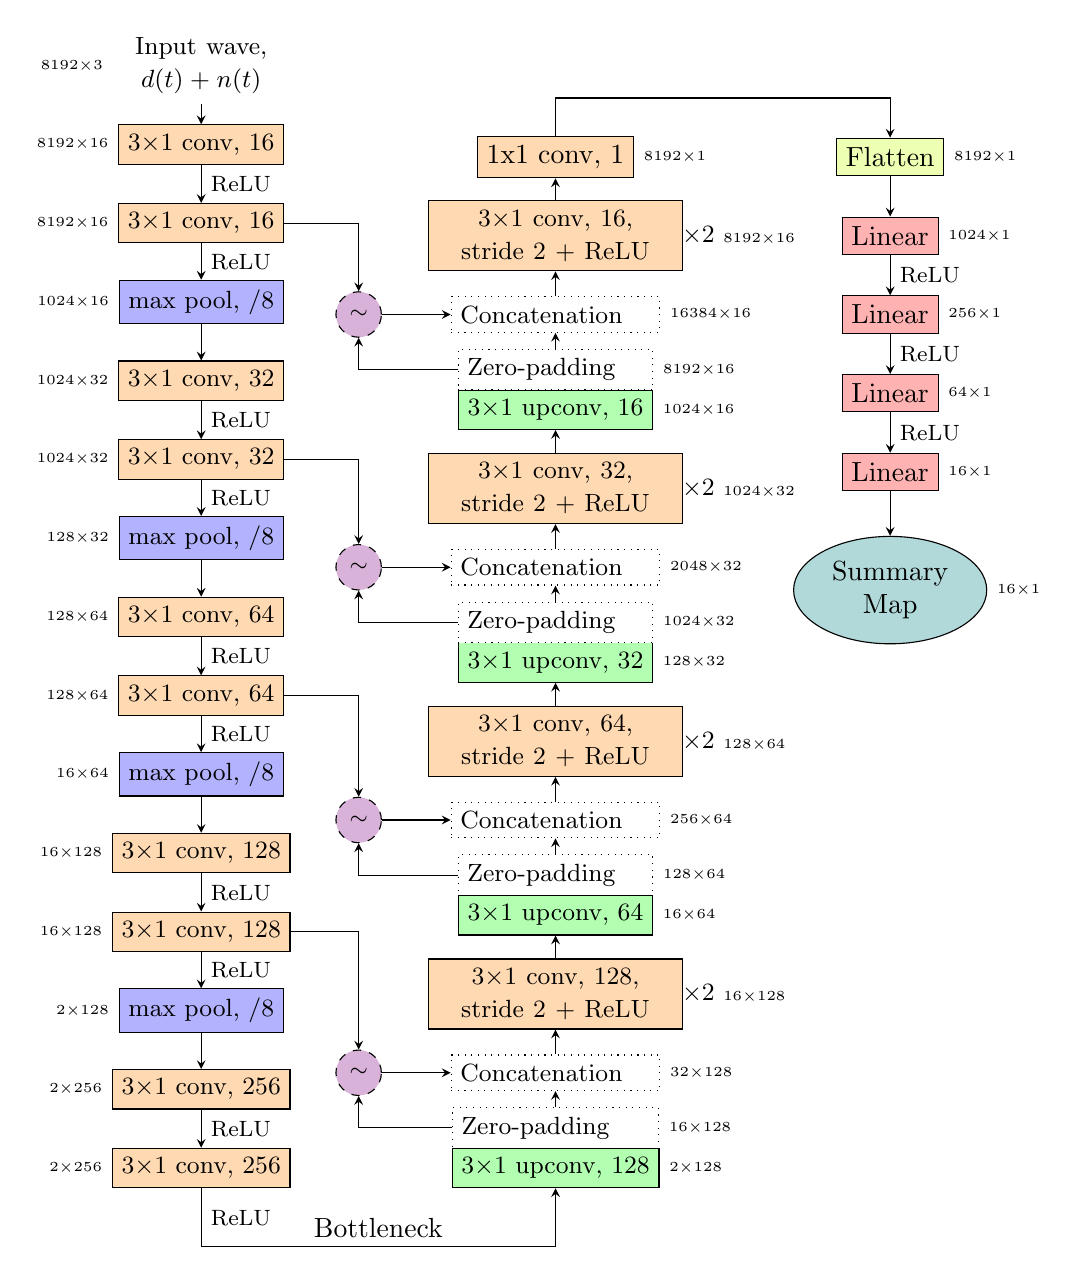
\begin{tikzpicture}[node distance=1.0cm]
		
    %%% NODES
    
    \node (input) [input, label=west:\tiny 8192$\times$3, text width=2cm] {\small Input wave, $d(t)+n(t)$};

    \node (conv1) [conv, below of=input, label=west:\tiny 8192$\times$16] {\small 3$\times$1 conv, 16};
    \node (conv2) [conv, below of=conv1, label=west:\tiny 8192$\times$16] {\small 3$\times$1 conv, 16};
    
    \node (pool1) [pool, below of=conv2, label=west:\tiny 1024$\times$16] {\small max pool, /8};
    
    \node (conv3) [conv, below of=pool1, label=west:\tiny 1024$\times$32] {\small 3$\times$1 conv, 32};
    \node (conv4) [conv, below of=conv3, label=west:\tiny 1024$\times$32] {\small 3$\times$1 conv, 32};
    
    \node (pool2) [pool, below of=conv4, label=west:\tiny 128$\times$32] {\small max pool, /8};
    
    \node (conv5) [conv, below of=pool2, label=west:\tiny 128$\times$64] {\small 3$\times$1 conv, 64};
    \node (conv6) [conv, below of=conv5, label=west:\tiny 128$\times$64] {\small 3$\times$1 conv, 64};
    
    \node (pool3) [pool, below of=conv6, label=west:\tiny 16$\times$64] {\small max pool, /8};
    
    \node (conv7) [conv, below of=pool3, label=west:\tiny 16$\times$128] {\small 3$\times$1 conv, 128};
    \node (conv8) [conv, below of=conv7, label=west:\tiny 16$\times$128] {\small 3$\times$1 conv, 128};
    
    \node (pool4) [pool, below of=conv8, label=west:\tiny 2$\times$128] {\small max pool, /8};

    \node (conv9) [conv, below of=pool4, label=west:\tiny 2$\times$256] {\small 3$\times$1 conv, 256};
    \node (conv10) [conv, below of=conv9, label=west:\tiny 2$\times$256] {\small 3$\times$1 conv, 256};
    
    %%%%%
    
    \node (upconv1) [upconv, right of=conv10, label=east:\tiny 2$\times$128, xshift=3.5cm] {\small 3$\times$1 upconv, 128};
    \node (zp1) [concat, above of=upconv1, label=east:\tiny 16$\times$128, yshift=-0.49cm] {\small Zero-padding \hspace{0.4cm} };
    \node (concat1) [concat, above of=zp1, label=east:\tiny 32$\times$128, yshift=-0.3cm] {\small Concatenation \hspace{0.25cm} };
    \node (upconvrelu1) [convx2, text width=3cm, above of=concat1, label=east:\small \hspace{-0.25cm} $\times$2 \tiny 16$\times$128] {\small 3$\times$1 conv, 128, stride 2 + ReLU};
    
    \node (AG1) [AG, left of=concat1, xshift=-1.5cm] {\footnotesize $\sim$};

    \node (upconv2) [upconv, above of=upconvrelu1, label=east:\tiny 16$\times$64] {\small 3$\times$1 upconv, 64};
    \node (zp2) [concat, above of=upconv2, label=east:\tiny 128$\times$64, yshift=-0.49cm] {\small Zero-padding \hspace{0.25cm} };
    \node (concat2) [concat, above of=zp2, label=east:\tiny 256$\times$64, yshift=-0.3cm] {\small Concatenation \hspace{0.25cm} };
    \node (upconvrelu2) [convx2, text width=3cm, above of=concat2, label=east:\small \hspace{-0.25cm} $\times$2 \tiny 128$\times$64] {\small 3$\times$1 conv, 64, stride 2 + ReLU};
    
    \node (AG2) [AG, left of=concat2, xshift=-1.5cm] {\footnotesize $\sim$};

    \node (upconv3) [upconv, above of=upconvrelu2, label=east:\tiny 128$\times$32] {\small 3$\times$1 upconv, 32};
    \node (zp3) [concat, above of=upconv3, label=east:\tiny 1024$\times$32, yshift=-0.49cm] {\small Zero-padding \hspace{0.25cm} };
    \node (concat3) [concat, above of=zp3, label=east:\tiny 2048$\times$32, yshift=-0.3cm] {\small Concatenation \hspace{0.25cm} };
    \node (upconvrelu3) [convx2, text width=3cm, above of=concat3, label=east:\small \hspace{-0.25cm} $\times$2 \tiny 1024$\times$32] {\small 3$\times$1 conv, 32, stride 2 + ReLU};
    
    \node (AG3) [AG, left of=concat3, xshift=-1.5cm] {\footnotesize $\sim$};
    
    \node (upconv4) [upconv, above of=upconvrelu3, label=east:\tiny 1024$\times$16] {\small 3$\times$1 upconv, 16};
    \node (zp4) [concat, above of=upconv4, label=east:\tiny 8192$\times$16, yshift=-0.49cm] {\small Zero-padding \hspace{0.25cm} };
    \node (concat4) [concat, above of=zp4, label=east:\tiny 16384$\times$16, yshift=-0.3cm] {\small Concatenation \hspace{0.25cm} };
    \node (upconvrelu4) [convx2, text width=3cm, above of=concat4, label=east:\small \hspace{-0.25cm} $\times$2 \tiny 8192$\times$16] {\small 3$\times$1 conv, 16, stride 2 + ReLU};
    
    \node (AG4) [AG, left of=concat4, xshift=-1.5cm] {\footnotesize $\sim$};

    \node (outconv) [outconv, above of=upconvrelu4, label=east:\tiny 8192$\times$1] {1x1 conv, 1};
    
    %%%
    
    \node (flatten) [flatten, right of=outconv, label=east:\tiny 8192$\times$1, xshift=3.25cm] {Flatten};
    \node (fc1) [fc, below of=flatten, label=east:\tiny 1024$\times$1] {Linear};
    \node (fc2) [fc, below of=fc1, label=east:\tiny 256$\times$1] {Linear};
    \node (fc3) [fc, below of=fc2, label=east:\tiny 64$\times$1] {Linear};
    \node (fc4) [fc, below of=fc3, label=east:\tiny 16$\times$1] {Linear};
    \node (summary) [summary, below of=fc4, label=east:\tiny 16$\times$1, yshift=-0.5cm] {Summary Map};
    
    %%% EDGES
                
    \draw [arrow_unet] (input) -- node[anchor=west]{}(conv1);
    
    \draw [arrow_unet] (conv1) -- node[anchor=west]{\footnotesize ReLU}(conv2);
    \draw [arrow_unet] (conv2) -- node[anchor=west]{\footnotesize ReLU}(pool1);
    \draw [arrow_unet] (pool1) -- node[anchor=west]{}(conv3);
    \draw [arrow_unet] (conv3) -- node[anchor=west]{\footnotesize ReLU}(conv4);
    \draw [arrow_unet] (conv4) -- node[anchor=west]{\footnotesize ReLU}(pool2);
    \draw [arrow_unet] (pool2) -- node[anchor=west]{}(conv5);
    \draw [arrow_unet] (conv5) -- node[anchor=west]{\footnotesize ReLU}(conv6);
    \draw [arrow_unet] (conv6) -- node[anchor=west]{\footnotesize ReLU}(pool3);
    \draw [arrow_unet] (pool3) -- node[anchor=west]{}(conv7);
    \draw [arrow_unet] (conv7) -- node[anchor=west]{\footnotesize ReLU}(conv8);
    \draw [arrow_unet] (conv8) -- node[anchor=west]{\footnotesize ReLU}(pool4);
    \draw [arrow_unet] (pool4) -- node[anchor=west]{}(conv9);
    \draw [arrow_unet] (conv9) -- node[anchor=west]{\footnotesize ReLU}(conv10);
    
    \draw [arrow_unet] (conv10) -- +(0,-1) node[pos=0.5, right]{\footnotesize ReLU} -| node[pos=0.25, above]{Bottleneck}(upconv1);
    
    %%%
    
    \draw [arrow_unet] (zp1) -| node[anchor=east]{}(AG1);			
    \draw [arrow_unet] (conv8) -| node[anchor=west]{}(AG1);
    \draw [arrow_unet] (AG1) -- node[anchor=west]{}(concat1);
    
    \draw [arrow_unet] (zp1) -- node[anchor=west]{}(concat1);
    \draw [arrow_unet] (concat1) -- node[anchor=west]{}(upconvrelu1);			
    \draw [arrow_unet] (upconvrelu1) -- node[anchor=west]{}(upconv2);			
    
    \draw [arrow_unet] (zp2) -| node[anchor=east]{}(AG2);			
    \draw [arrow_unet] (conv6) -| node[anchor=west]{}(AG2);
    \draw [arrow_unet] (AG2) -- node[anchor=west]{}(concat2);
    
    \draw [arrow_unet] (zp2) -- node[anchor=west]{}(concat2);
    \draw [arrow_unet] (concat2) -- node[anchor=west]{}(upconvrelu2);			
    \draw [arrow_unet] (upconvrelu2) -- node[anchor=west]{}(upconv3);	
    
    \draw [arrow_unet] (zp3) -| node[anchor=east]{}(AG3);			
    \draw [arrow_unet] (conv4) -| node[anchor=west]{}(AG3);
    \draw [arrow_unet] (AG3) -- node[anchor=west]{}(concat3);
    
    \draw [arrow_unet] (zp3) -- node[anchor=west]{}(concat3);
    \draw [arrow_unet] (concat3) -- node[anchor=west]{}(upconvrelu3);			
    \draw [arrow_unet] (upconvrelu3) -- node[anchor=west]{}(upconv4);	
    
    \draw [arrow_unet] (zp4) -| node[anchor=east]{}(AG4);			
    \draw [arrow_unet] (conv2) -| node[anchor=west]{}(AG4);
    \draw [arrow_unet] (AG4) -- node[anchor=west]{}(concat4);
    
    \draw [arrow_unet] (zp4) -- node[anchor=west]{}(concat4);
    \draw [arrow_unet] (concat4) -- node[anchor=west]{}(upconvrelu4);			
    \draw [arrow_unet] (upconvrelu4) -- node[anchor=west]{}(outconv);	
    
    %%%
    
    \draw [arrow_unet] (outconv) -- +(0,0.75) -| node[anchor=west]{}(flatten);
    \draw [arrow_unet] (flatten) -- node[anchor=west]{}(fc1);
    \draw [arrow_unet] (fc1) -- node[anchor=west]{\footnotesize ReLU}(fc2);
    \draw [arrow_unet] (fc2) -- node[anchor=west]{\footnotesize ReLU}(fc3);
    \draw [arrow_unet] (fc3) -- node[anchor=west]{\footnotesize ReLU}(fc4);
    \draw [arrow_unet] (fc4) -- node[anchor=west]{}(summary);
			
	\end{tikzpicture}	
 
\caption{The architecture of Attention U-Net as implemented for the processing of the time domain signal. The frequency domain follows the same architecture, but the max pooling layer is a factor of 2, and the initial input wave is 4097$\times$6. The difference between Attention U-Net and original U-Net is the addition of the Attention gates ($\sim$) in the skip layers.}
\label{fig:Attention_UNet_arch}
 
\end{figure}

\end{appendices}


\end{document}

%%%%%%%%%%%%%%%%%%%%%%%%%%%%%%%%%%%%%%%%%%%%%%%%%%%%%%%%%%%%%%%%%%%%%%%%%%%%%%%%
%%%%%%%%%%%%%%%%%%%%%%%%%%%%%%%%%%%%%%%%%%%%%%%%%%%%%%%%%%%%%%%%%%%%%%%%%%%%%%%%